


%%%%%%%%%%%%%%%%%%%%%%%%%%%%%%%%%%%%%%%%%
% Beamer Presentation
% LaTeX Template
% Version 1.0 (10/11/12)
%
% This template has been downloaded from:
% http://www.LaTeXTemplates.com
%
% License:
% CC BY-NC-SA 3.0 (http://creativecommons.org/licenses/by-nc-sa/3.0/)
%
%%%%%%%%%%%%%%%%%%%%%%%%%%%%%%%%%%%%%%%%%

%----------------------------
%	PACKAGES AND THEMES
%----------------------------

\documentclass{beamer}

\mode<presentation> {

% The Beamer class comes with a number of default slide themes
% which change the colors and layouts of slides. Below this is a list
% of all the themes, uncomment each in turn to see what they look like.

%\usetheme{default}
%\usetheme{AnnArbor}
%\usetheme{Antibes}
%\usetheme{Bergen}
%\usetheme{Berkeley}
%\usetheme{Berlin}
%\usetheme{Boadilla}
%\usetheme{CambridgeUS}
%\usetheme{Copenhagen}
% \usetheme{Darmstadt}
% \usetheme{Dresden}
%\usetheme{Frankfurt}
%\usetheme{Goettingen}
%\usetheme{Hannover}
%\usetheme{Ilmenau}
%\usetheme{JuanLesPins}
%\usetheme{Luebeck}
%\usetheme{Madrid}
%\usetheme{Malmoe}
%\usetheme{Marburg}
%\usetheme{Montpellier}
%\usetheme{PaloAlto}
%\usetheme{Pittsburgh}
%\usetheme{Rochester}
%\usetheme{Singapore}
% \usetheme{Szeged}
\usetheme{Warsaw}

% As well as themes, the Beamer class has a number of color themes
% for any slide theme. Uncomment each of these in turn to see how it
% changes the colors of your current slide theme.

% \usecolortheme{albatross}
% \usecolortheme{beaver}
% \usecolortheme{beetle}
% \usecolortheme{crane}
% \usecolortheme{dolphin}
% \usecolortheme{dove}
% \usecolortheme{fly}
% \usecolortheme{lily}
% \usecolortheme{orchid}
\usecolortheme{rose} % #Kawasaki
% \usecolortheme{seagull}
% \usecolortheme{seahorse}
% \usecolortheme{whale}
% \usecolortheme{wolverine}

%\setbeamertemplate{footline} % To remove the footer line in all slides uncomment this line
%\setbeamertemplate{footline}[page number] % To replace the footer line in all slides with a simple slide count uncomment this line

%\setbeamertemplate{navigation symbols}{} % To remove the navigation symbols from the bottom of all slides uncomment this line
}

\usepackage{graphicx} % Allows including images
\usepackage{booktabs} % Allows the use of \toprule, \midrule and \bottomrule in tables

%---------------------------
%	TITLE PAGE
%---------------------------

\title[Origami]{The Mathematics of Origami} % The short title appears at the bottom of every slide, the full title is only on the title page

\author[T. Bertschinger, J. Slote, C. Spencer, S. Vinitsky]{Thomas Bertschinger, Joseph Slote, Claire Spencer, \\ \& Samuel Vinitsky} % Your name
\institute[Carleton] % Your institution as it will appear on the bottom of every slide, may be shorthand to save space
{
Carleton College \\ % Your institution for the title page
\medskip
}
\date{\today} % Date, can be changed to a custom date

\newcommand{\paws}{\pause}

\begin{document}

\begin{frame}
\titlepage % Print the title page as the first slide
\end{frame}

\begin{frame}
\frametitle{Overview} % Table of contents slide, comment this block out to remove it
\tableofcontents % Throughout your presentation, if you choose to use \section{} and \subsection{} commands, these will automatically be printed on this slide as an overview of your presentation
\end{frame}

%````````````````````'''''''''''''''''''%
%~~~~~~~~ PRESENTATION SLIDES ~~~~~~~~~~%
%'''''''''''''''''''````````````````````%

\section{Origami Constructions}

\begin{frame}
\frametitle{Axioms of Origami}
\begin{block}{General}
\begin{enumerate}
\item[i.]
Brief History
\item[ii.]
Independence
\end{enumerate}
\end{block}
\end{frame}

\begin{frame}
\frametitle{Axioms of Origami}
\begin{block}{Seven Axioms of Origami}
\begin{enumerate}
\item[i.]
Given two points $p_1$ and $p_2$, we can fold a line connecting them.
\item[ii.]
Given two points $p_1$ and $p_2$, we can fold $p_1$ onto $p_2$.
\item[iii.]
Given two lines $l_1$ and $l_2$, we can fold line $l_1$ onto $l_2$.
\item[iv.]
Given a point $p_1$ and a line $l_1$, we can make a fold perpendicular to $l_1$ passing through the point $p_1$.
\end{enumerate}
\end{block}
\end{frame}

\begin{frame}
\frametitle{Axioms of Origami}
\begin{block}{Seven Axioms of Origami}
\begin{enumerate}
\item[v.]
Given two points $p_1$ and $p_2$ and a line $l_1$, we can make a fold that places $p_1$ onto $l_1$ and passes through the point $p_2$.
\item[vi.]
Given two points $p_1$ and $p_2$ and two lines $l_1$ and $l_2$, we can make a fold that places p1 onto line $l_1$ and places $p_2$ onto line $l_2$.
\item[vii.]
Given a point $p_1$ and two lines $l_1$ and $l_2$, we can make a fold perpendicular to $l_2$ that places $p_1$ onto line $l_1$.
\end{enumerate}
\end{block}
\end{frame}

\begin{frame}
\frametitle{Axioms of Origami}
\begin{block}{Seven Axioms of Origami}
\begin{enumerate}
\item[i.]
The first six axioms allow all quadratic and cubic equations with rational coefficients to be solved.
\item[ii.]
They also allow two of the three problems of antiquity, the trisection of an angle and the doubling of the cube, to be constructed.
\end{enumerate}
\end{block}
\end{frame}

\begin{frame}
\frametitle{Greek Problems of Antiquity}
\begin{block}{Problems of Antiquity}
These were a trio of geometric problems whose solutions were attempted solely through the use of compass and straight-edge.
\begin{enumerate}
\item[i.]
Angle Trisection
\item[ii.]
Cube Duplication
\item[iii.]
Circle Squaring
\end{enumerate}
\end{block}
\end{frame}

\begin{frame}
\frametitle{Angle Trisection}
INCLUDE PARTIALLY FOLDED DIAGRAMS
\end{frame}

\begin{frame}
\frametitle{Cube Duplication}
INCLUDE PARTIALLY FOLDED DIAGRAMS
\begin{enumerate}
\item[i.]
$\frac{\alpha}{\beta} = \sqrt[3]{2}$
\item[ii.]
Thus, a cube with a side length $\alpha$ will have twice the volume of a cube with side length $\beta$.
\end{enumerate}
\end{frame}

\begin{frame}
\frametitle{Squaring the Circle}
\begin{enumerate}
\item[i.]
Impossible
\item[ii.]
$\pi$
\end{enumerate}
\end{frame}

\begin{frame}
\frametitle{Constructability}
\begin{block}{Constructible Numbers}
\begin{enumerate}
\item[i.]
Given two points $p_0$ and $p_1$, construct a third point $p_1'$ a distance $|p_0 p_1|$ from point $p_0$ such that $\overline{p_0 p_1'}$ is perpendicular to $\overline{p_0 p_1}$.
\item[ii.]
Given two points $p_0$ and $p_1$, a third point $p_2$ can be constructed such that $p_2$ is collinear with $p_0$ and $p_1$, thus $|p_0 p_1| = |p_1 p_2|$.
\end{enumerate}
\end{block}
\end{frame}

\begin{frame}
\frametitle{Constructability}
\begin{block}{Constructible Numbers}
\begin{enumerate}
\item[iii.]
Given two constructible numbers $\alpha$ and $\beta$, we can construct $\frac{\alpha}{\beta}$, their ratio.
\item[iv.]
Given two constructible numbers $\alpha$ and $\beta$, we can construct their sum $\alpha + \beta$ or their difference $\alpha - \beta$.
\item[v.]
Given two constructible numbers $\alpha$ and $\beta$, we can construct $\alpha\beta$, their product.
\end{enumerate}
\end{block}
\end{frame}

\begin{frame}
\frametitle{Constructability}
Given two constructible numbers $\alpha$ and $\beta$, we can construct $\frac{\alpha}{\beta}$, their ratio.

INCLUDE PARTIALLY FOLDED DIAGRAMS AS WELL AS FINAL FOLDED DIAGRAM
\end{frame}

\begin{frame}
\frametitle{Constructability}
\begin{block}{Constructible Numbers}
\begin{enumerate}
\item[i.]
Since the set of constructible numbers is closed under addition, subtraction, multiplication, and division, it can be concluded that the set of constructible numbers form a field.
\item[ii.]
Ultimately, the field of origami constructible numbers are closed under taking both square roots and cube roots.
\item[iii.]
The construction of the square root of any constructible number implies the field of origami constructible numbers contains the field of compass and straightedge constructible numbers.
\end{enumerate}
\end{block}
\end{frame}

\begin{frame}
\frametitle{Future Work}
\begin{enumerate}
\item[i.]
Efficiency
\item[ii.]
Optimality
\end{enumerate}
\end{frame}

\subsection{Axioms, Euclid \&c.}

\section{The Basics of Foldability}

\begin{frame}
\frametitle{Foldability}
\begin{block}{}
An example of a crease pattern:
\end{block}
\begin{center}
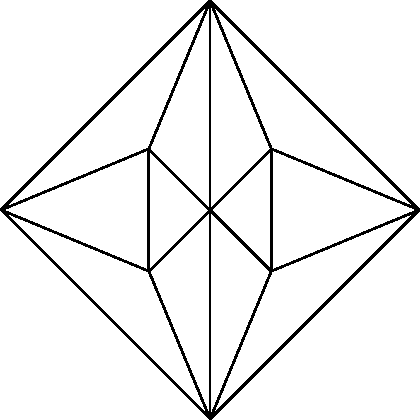
\includegraphics[width=.5\textwidth]{sam_images/bird-base-unfolded.pdf}
\end{center}
\end{frame}

\begin{frame}
\frametitle{Foldability}
\begin{block}{Crease Assignments}
A crease pattern doesn't contain all the information about a model, however. 
\end{block}
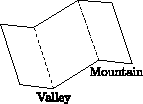
\includegraphics[width=.5\textwidth]{foldability_pix/mountain-valley.pdf}
\end{frame}

\begin{frame}
\frametitle{Foldability}
\begin{center}
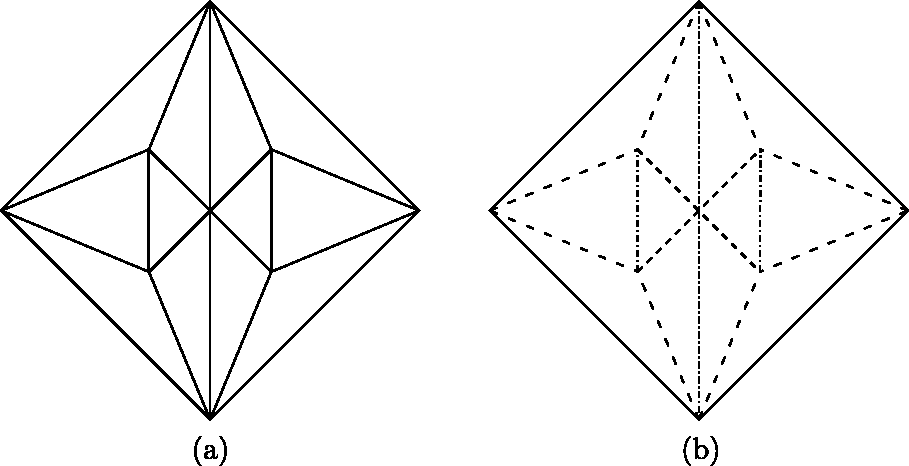
\includegraphics[width=\textwidth]{foldability_pix/bird_base.pdf}
\end{center}
\end{frame}

\begin{frame}
\frametitle{Foldability}
\begin{block}{Two questions}
For a given crease pattern,
\begin{enumerate}
\item[i.]
is there a way to fold it flat?
\item[ii.]
is there a way to fold it at all?
\end{enumerate}
\end{block}
\end{frame}

\subsection{Local Flat Foldability}

\begin{frame}
\frametitle{Kawasaki's Theorem}
\begin{block}{Theorem}
The alternate angles around a vertex must sum to $180^\circ$.
\end{block}
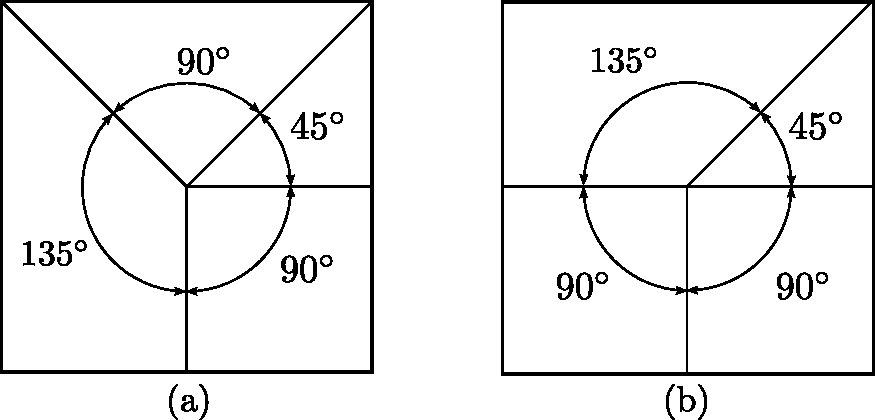
\includegraphics[width=\textwidth]{foldability_pix/kawasaki_passfail.pdf}
\end{frame}
\begin{frame}
\frametitle{Kawasaki's Theorem}
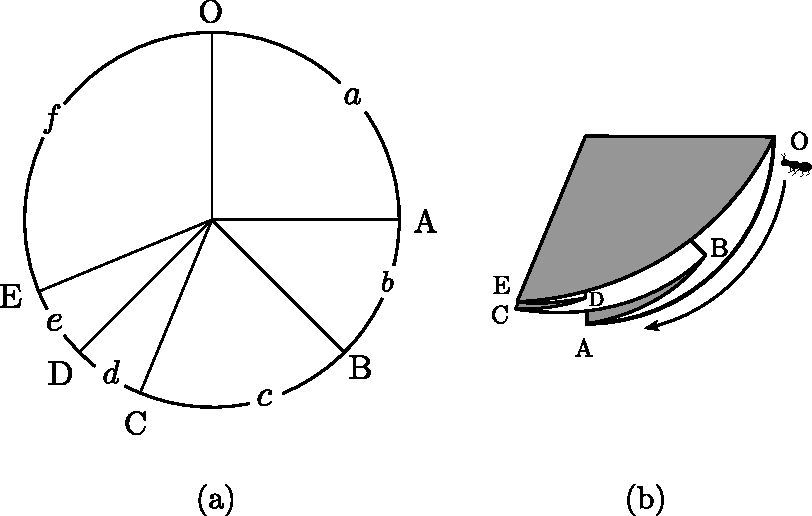
\includegraphics[width=\textwidth]{foldability_pix/kawasaki_proof.pdf}
\end{frame}

\begin{frame}
\frametitle{Maekawa's Theorem}
\begin{block}{Theorem}
The sum of mountain + valley is $\pm 2$. 
\end{block}
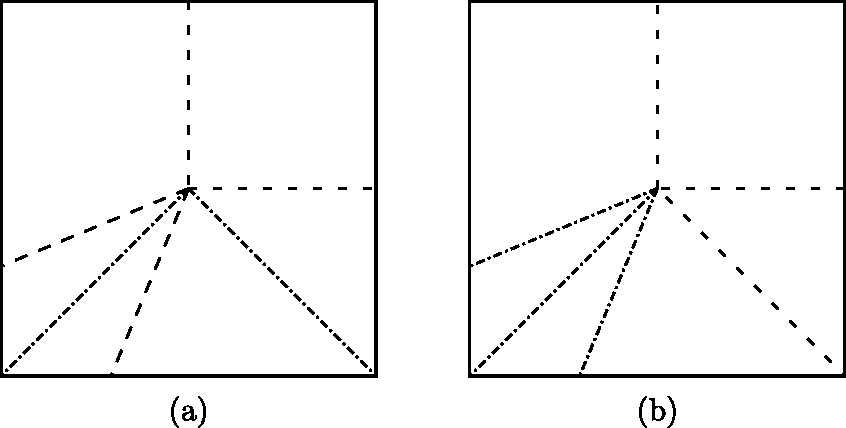
\includegraphics[width=\textwidth]{foldability_pix/maekawa_img.pdf}
\end{frame}
\begin{frame}
\frametitle{Maekawa's Theorem}
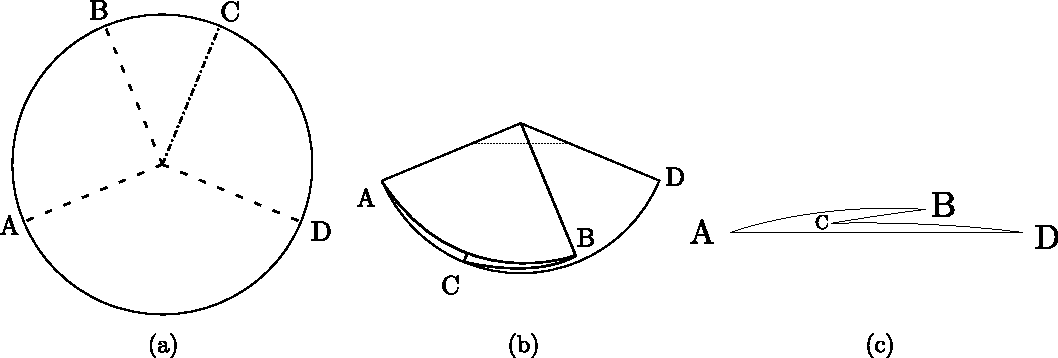
\includegraphics[width=\textwidth]{foldability_pix/maekawa_proof.pdf}
\end{frame}

\begin{frame}
\frametitle{More Complicated Crease Patterns}
\begin{block}{}
How can we determine flat foldability for a more complicated pattern?
\newline
(a picture of a complicated crease pattern)
\end{block}
\end{frame}

\begin{frame}
\frametitle{More Complicated Crease Patterns}
\begin{block}{}
Here's a crease pattern that can't fold flat!
\end{block}
(a picture of the thing)

\end{frame}

%% BEFORE GOING ON %%
%___ "we are going ii introduce a theorem _____%
%___ that ties together origmi and topology ___%
%___ but first we gotta get you up to speed ___%
%___ on foldings and knots. ___________________%
%% WE MAY NOW CONTINUE %%

\subsection{General Foldability}

\begin{frame}
\frametitle{Foldings}

\begin{block}{}
How can we capture the notion of a folded paper? 
\end{block}

\pause
\begin{columns}[c]
\column{.45\textwidth}
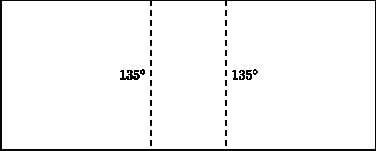
\includegraphics[width=\textwidth]{foldability_pix/unfolded.pdf}

\pause
\column{.45\textwidth}
%\includegraphics[width=\textwidth]{}
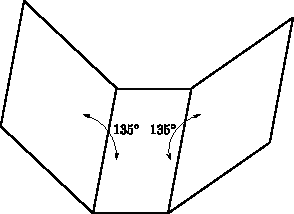
\includegraphics[width=\textwidth]{knot_pix/folded-valid.pdf}
\end{columns}
\end{frame}


\begin{frame}
\frametitle{An Invalid Folding}
\begin{columns}[c]
\column{.45\textwidth}
This folding has self-intersection.
\column{.45\textwidth}
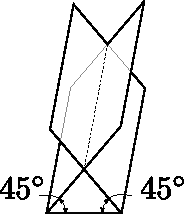
\includegraphics[width=.6\textwidth]{knot_pix/folded-invalid.pdf}
\end{columns}
\end{frame}

\begin{frame}
\frametitle{Valid Foldings}
\begin{block}{}
A valid folding is one that doesn't cause any self-intersecton. 
\end{block}
\begin{columns}[c]
\column{.45\textwidth}
\begin{center}
Valid
\end{center}
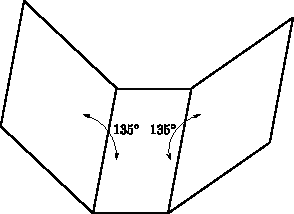
\includegraphics[width=\textwidth]{knot_pix/folded-valid.pdf}
\column{.45\textwidth}
\begin{center}
Invalid

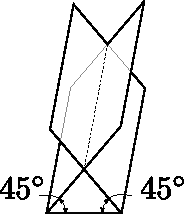
\includegraphics[width=.4\textwidth]{knot_pix/folded-invalid.pdf}
\end{center}
\end{columns}
\end{frame}

\begin{frame}
\frametitle{Drawing pictures on Crease Patterns}
\begin{block}{Question}
If we draw something on the flat piece of paper before folding it up, what can happen when we fold it? 
\end{block}
\pause
\begin{columns}[c]
\column{.45\textwidth}
We'll see what happens when we draw Jordan curves on the crease patterns, like the picture on the right. 
\column{.45\textwidth}
%\includegraphics[width=\textwidth]{}
(a picture of a Jordan curve on a crease pattern)
\end{columns}
\end{frame}

\subsection{Knots}

\begin{frame}
\frametitle{Knot Theory 101}
\begin{block}{What is a knot?}
Here's how we think of a knot mathematically. 
\end{block}
\end{frame}

\begin{frame}
\frametitle{Knot Theory 101}
\begin{columns}[c]
\column{.45\textwidth}
\centering
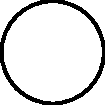
\includegraphics[width=.8\textwidth]{knot_pix/unknot.pdf}
\column{.45\textwidth}
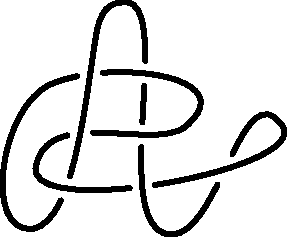
\includegraphics[width=\textwidth]{knot_pix/untrivial-unknot.pdf}
\end{columns}
\end{frame}

\begin{frame}
\frametitle{Knot Theory 101}
\begin{columns}[c]
\column{.45\textwidth}
This is the \textit{trefoil knot}. We can't ``untangle'' it, no matter how hard we try. 
\column{.45\textwidth}
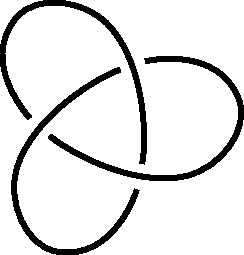
\includegraphics[width=\textwidth]{knot_pix/trefoil}
\end{columns}
\end{frame}


\begin{frame}
\frametitle{Connecting Topology and Origami}
\begin{theorem}
A folding of a crease pattern $C$ is valid if and only if every Jordan curve embedded in the paper before folding is mapped to the unknot after folding. 
\end{theorem}
\pause
It's obvious that the first direction is true (we can't cause knot without invalid folding)
\end{frame}

\begin{frame}
\frametitle{Connecting Topology and Origami}
\begin{block}{}
Invalid folding means intersection. 
\end{block}
\begin{columns}[c]
\column{.5\textwidth}
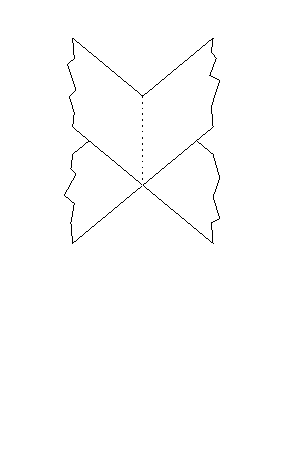
\includegraphics[width=.8\textwidth]{knot_pix/finding-ribbon_1.pdf}
\column{.5\textwidth}
\end{columns}
\end{frame}

\begin{frame}
\frametitle{Connecting Topology and Origami}
\begin{block}{}
We can connect up the paper like this. 
\end{block}
\begin{columns}[c]
\column{.5\textwidth}
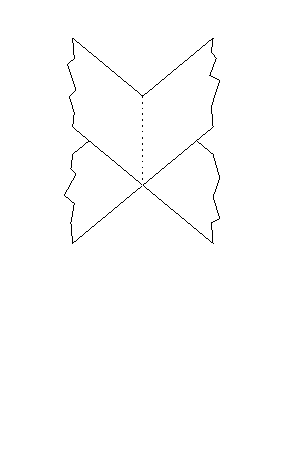
\includegraphics[width=.8\textwidth]{knot_pix/finding-ribbon_1.pdf}
\column{.5\textwidth}
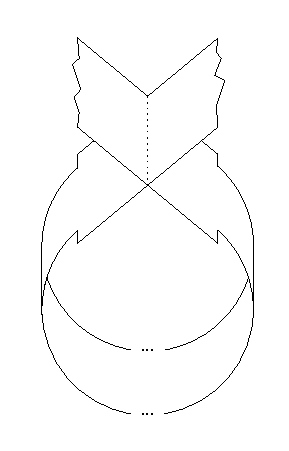
\includegraphics[width=.8\textwidth]{knot_pix/finding-ribbon_2.pdf}
\end{columns}
\end{frame}

\begin{frame}
\frametitle{Connecting Topology and Origami}
\begin{block}{}
We can draw a curve like this. 
\end{block}
\begin{center}
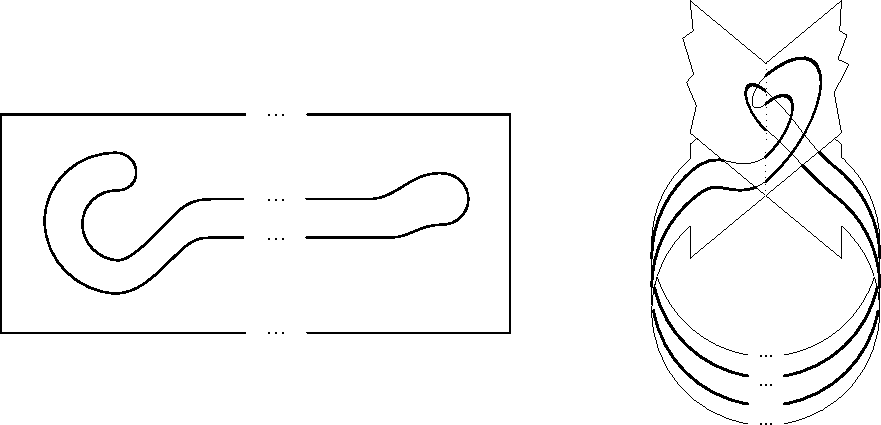
\includegraphics[width=.7\textwidth]{knot_pix/marking-jordan.pdf}
\end{center}
\end{frame}

\begin{frame}
\frametitle{Connecting Topology and Origami}
\begin{block}{}
Is it a knot?
\end{block}
\begin{columns}[c]
\column{.25\textwidth}
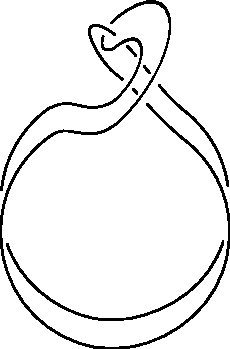
\includegraphics[width=.9\textwidth]{knot_pix/knot_1.pdf}
\column{.25\textwidth}
\pause
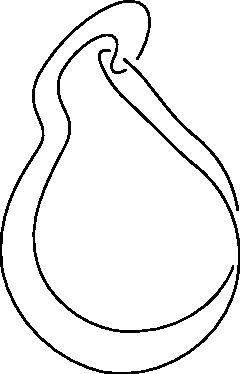
\includegraphics[width=.9\textwidth]{knot_pix/knot_2.pdf}
\column{.25\textwidth}
\pause
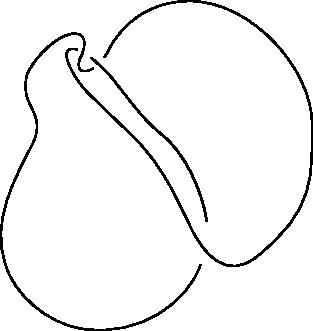
\includegraphics[width=.7\textwidth]{knot_pix/knot_3.pdf}
\column{.25\textwidth}
\pause
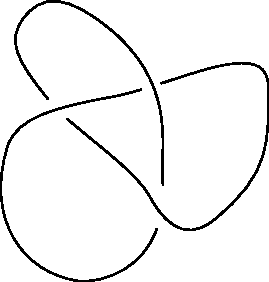
\includegraphics[width=.7\textwidth]{knot_pix/knot_4.pdf}

\end{columns}
\end{frame}

\begin{frame}
\frametitle{Connecting Topology and Origami}
\begin{block}{}
We've skipped over some details, but you can ask us if you don't believe our proof. 
\end{block}
\end{frame}


%%%%%%%%%%%%%%%%%%%%%%%%%%%%%%%%%%%%%%%%%%%%%%%%%%%%%%%%%%%%%%%%%%%%%%%%
%%%%%%%%%%%%%%%%%%%%%%%%%%%%%%%%%%%%%%%%%%%%%%%%%%%%%%%%%%%%%%%%%%%%%%%%
%%%%%%%%%%%%%%%%%%%%%%%%%%%%%%%%%%%%%%%%%%%%%%%%%%%%%%%%%%%%%%%%%%%%%%%%
%%%%%%%%%%%%%%%%%%%%%%%%%%%%%%%%%%%%%%%%%%%%%%%%%%%%%%%%%%%%%%%%%%%%%%%%
%%%%%%%%%%%%%%%%%%%%%%%%%%%%%%%%%%%%%%%%%%%%%%%%%%%%%%%%%%%%%%%%%%%%%%%%
%%%%%%%%%%%%%%%%%%%%%%%%%%%%%%%%%%%%%%%%%%%%%%%%%%%%%%%%%%%%%%%%%%%%%%%%

\section{Map Folding: An Open Problem}

\def\O{\mathcal{L}}

\subsection{Overview}
%%%%%%%%%%%%%%%%%%%%%%%%%%%%%%%%%%%%%%%%%%%%%%%%%%%%%%%%%%%%%%%%%%%%%%%%
\begin{frame} 
\frametitle{Determining flat-foldability}

\begin{block}{Question:}
Is this crease pattern flat-foldable?
\end{block} 

\bigskip

\begin{columns}[c]
\column{.45\textwidth}
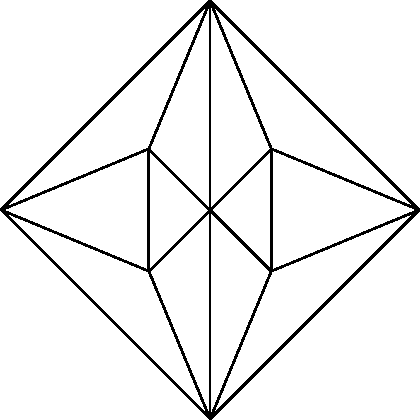
\includegraphics[width=\textwidth]{sam_images/bird-base-unfolded.pdf}

\pause

\column{.25\textwidth}
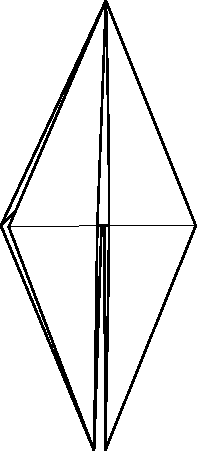
\includegraphics[height=.5\textheight]{sam_images/bird-base-folded.pdf}

\end{columns}

\end{frame}

%%%%%%%%%%%%%%%%%%%%%%%%%%%%%%%%%%%%%%%%%%%%%%%%%%%%%%%%%%%%%%%%%%%%%%%%
\begin{frame}
\frametitle{Introduction to Maps}

\begin{columns}[c]
\column{.3\textwidth}
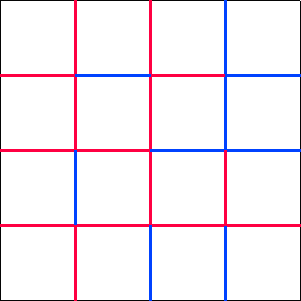
\includegraphics[width=\textwidth]{sam_images/yes-map-1.pdf}

\bigskip
\bigskip

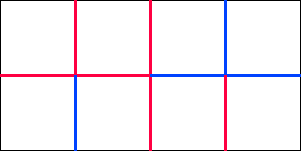
\includegraphics[width=\textwidth]{sam_images/yes-map-2.pdf}

\column{.3\textwidth}
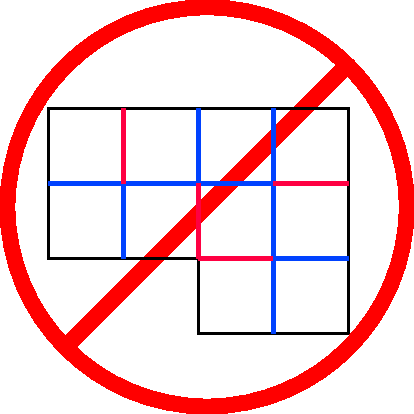
\includegraphics[width=\textwidth]{sam_images/no-map.pdf}

\bigskip

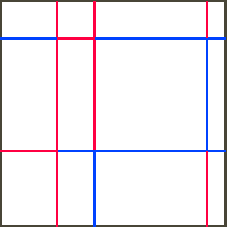
\includegraphics[width=\textwidth]{sam_images/no-map-2.pdf}

\end{columns}

\end{frame}
%%%%%%%%%%%%%%%%%%%%%%%%%%%%%%%%%%%%%%%%%%%%%%%%%%%%%%%%%%%%%%%%%%%%%%%%
\begin{frame}
\frametitle{Introduction to Maps}

\begin{columns}[c]
\column{.75\textwidth}
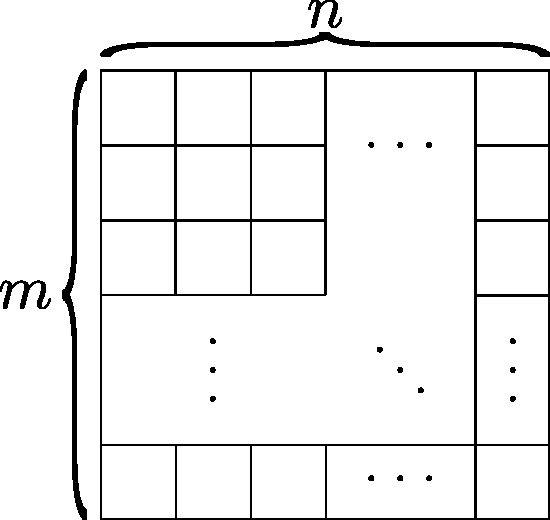
\includegraphics[height=.8\textheight]{sam_images/general-map.pdf}
\end{columns}

\end{frame}

%%%%%%%%%%%%%%%%%%%%%%%%%%%%%%%%%%%%%%%%%%%%%%%%%%%%%%%%%%%%%%%%%%%%%%%%
\begin{frame}
\frametitle{Map Folding: An Open Problem}

\begin{block}{Open Problem:}
How hard is it to determine whether or not a map is flat-foldable?
\end{block}

\bigskip
\bigskip
\bigskip

\pause
\begin{block}{Easier Problem:}
How hard is it to determine whether or not a map is \textit{flat-folded}?
\end{block}

\end{frame}
%%%%%%%%%%%%%%%%%%%%%%%%%%%%%%%%%%%%%%%%%%%%%%%%%%%%%%%%%%%%%%%%%%%%%%%%
\begin{frame}

\frametitle{Linear Orderings}

\begin{block}{Question:}
How can we represent a folded form?
\end{block}

\bigskip
\bigskip

\begin{columns}[c]
\column{.3\textwidth}
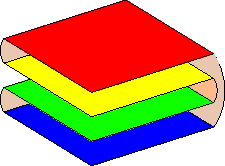
\includegraphics[height=.3\textheight]{sam_images/2x2-map-folded.pdf}

\pause

\column{.5\textwidth}

red $\rightarrow$ yellow $\rightarrow$ green $\rightarrow$ blue

\end{columns}

\end{frame}
%%%%%%%%%%%%%%%%%%%%%%%%%%%%%%%%%%%%%%%%%%%%%%%%%%%%%%%%%%%%%%%%%%%%%%%%
\begin{frame}

\frametitle{Linear Orderings}

\begin{block}{Question:}
How can we tell if a linear ordering is realizable by a given crease pattern?
\end{block}

\bigskip
\bigskip

\end{frame}

%%%%%%%%%%%%%%%%%%%%%%%%%%%%%%%%%%%%%%%%%%%%%%%%%%%%%%%%%%%%%%%%%%%%%%%%

\subsection{Linear Orderings}

\begin{frame}
\frametitle{Checkerboard Pattern}

\bigskip

\begin{columns}[c]
\column{.45\textwidth}
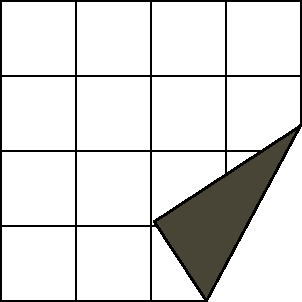
\includegraphics[width=\textwidth]{sam_images/checkerboard-1.pdf}

\pause

\column{.45\textwidth}
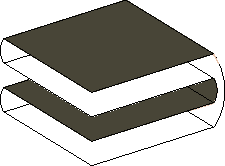
\includegraphics[width=\textwidth]{sam_images/checkerboard-2.pdf}

\end{columns}

\end{frame}
%%%%%%%%%%%%%%%%%%%%%%%%%%%%%%%%%%%%%%%%%%%%%%%%%%%%%%%%%%%%%%%%%%%%%%%%
\begin{frame}
\frametitle{Checkerboard Pattern}

\begin{block}{Goal:}
Label each face as being light-side or dark-side up in \textit{any} folding.
\end{block}

\bigskip

\begin{columns}[c]
\column{.45\textwidth}
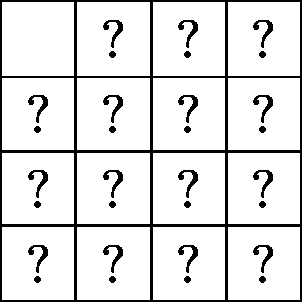
\includegraphics[width=\textwidth]{sam_images/checkerboard-3.pdf}

\pause

\column{.45\textwidth}
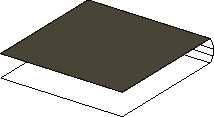
\includegraphics[width=.9\textwidth]{sam_images/checkerboard-3a.pdf}

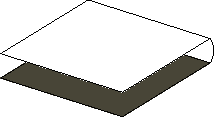
\includegraphics[width=.9\textwidth]{sam_images/checkerboard-3d.pdf}

\end{columns}

\end{frame}

%%%%%%%%%%%%%%%%%%%%%%%%%%%%%%%%%%%%%%%%%%%%%%%%%%%%%%%%%%%%%%%%%%%%%%%%
\begin{frame}
\frametitle{Checkerboard Pattern}

\begin{block}{Goal:}
Label each face as being light-side or dark-side up in \textit{any} folding.
\end{block}

\bigskip

\begin{columns}[c]
\column{.45\textwidth}
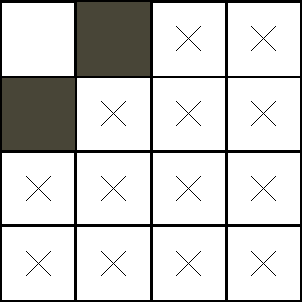
\includegraphics[width=\textwidth]{sam_images/checkerboard-3c.pdf}

\column{.45\textwidth}
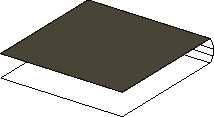
\includegraphics[width=.9\textwidth]{sam_images/checkerboard-3a.pdf}

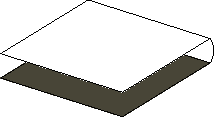
\includegraphics[width=.9\textwidth]{sam_images/checkerboard-3d.pdf}

\end{columns}

\end{frame}

%%%%%%%%%%%%%%%%%%%%%%%%%%%%%%%%%%%%%%%%%%%%%%%%%%%%%%%%%%%%%%%%%%%%%%%%
\begin{frame}
\frametitle{Checkerboard Pattern}

\begin{block}{Goal:}
Label each face as being light-side or dark-side up in \textit{any} folding.
\end{block}

\bigskip

\begin{columns}[c]
\column{.45\textwidth}
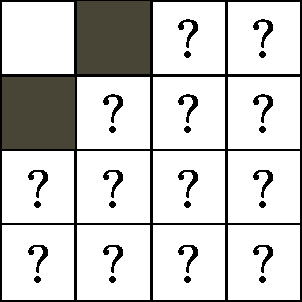
\includegraphics[width=\textwidth]{sam_images/checkerboard-3b.pdf}

\column{.45\textwidth}
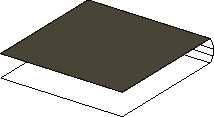
\includegraphics[width=.9\textwidth]{sam_images/checkerboard-3a.pdf}

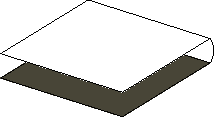
\includegraphics[width=.9\textwidth]{sam_images/checkerboard-3d.pdf}

\end{columns}

\end{frame}
%%%%%%%%%%%%%%%%%%%%%%%%%%%%%%%%%%%%%%%%%%%%%%%%%%%%%%%%%%%%%%%%%%%%%%%%
\begin{frame}
\frametitle{Checkerboard Pattern}

\begin{block}{Goal:}
Label each face as being light-side or dark-side up in \textit{any} folding.
\end{block}

\bigskip

\begin{columns}[c]
\column{.45\textwidth}
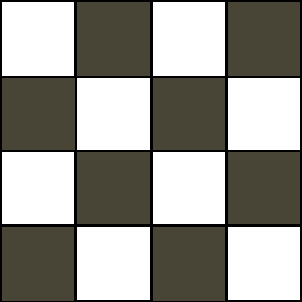
\includegraphics[width=\textwidth]{sam_images/checkerboard-complete.pdf}

\column{.45\textwidth}

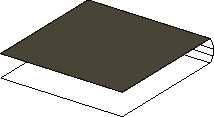
\includegraphics[width=.9\textwidth]{sam_images/checkerboard-3a.pdf}

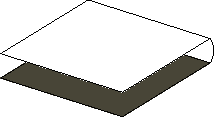
\includegraphics[width=.9\textwidth]{sam_images/checkerboard-3d.pdf}

\end{columns}

\end{frame}

%%%%%%%%%%%%%%%%%%%%%%%%%%%%%%%%%%%%%%%%%%%%%%%%%%%%%%%%%%%%%%%%%%%%%%%%


\begin{frame}
\frametitle{Partial Ordering}
\begin{block}{Definition:}
A \textit{partial ordering} $P$ on a set $S$ is a set of ordered pairs of elements of $S$ that orders some of the elements of $S$.
\end{block}

\medskip

\underline{Example:} \\

\smallskip
\pause

$S = \{a, b, c, d\}$ \\

\smallskip
\pause

A partial ordering $S$ might be $\{(a\rightarrow b),(c\rightarrow d)\}$. \\

\smallskip
\pause

In every linear ordering that satisfies $P$, we know $a\rightarrow b$ and $c\rightarrow d$. \\

\smallskip
\pause

Note however that there are many such linear orderings: \\

\smallskip
\pause

$a\rightarrow b\rightarrow c\rightarrow d$ \\
\pause
$a\rightarrow c\rightarrow b\rightarrow d$ \\
$c\rightarrow d \rightarrow a \rightarrow b$ \\
...

\end{frame}

%%%%%%%%%%%%%%%%%%%%%%%%%%%%%%%%%%%%%%%%%%%%%%%%%%%%%%%%%%%%%%%%%%%%%%%%

\begin{frame}
\frametitle{Partial Ordering}
\begin{block}{Goal:}
Use checkerboard pattern and crease assignments to tell, for each pair of adjacent faces, which face comes first in \textit{all} linear orderings.
\end{block}

\bigskip

\begin{columns}[c]
\column{.45\textwidth}
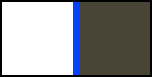
\includegraphics[width=\textwidth]{sam_images/cboard-mountain-tile.pdf}

\pause

\column{.45\textwidth}
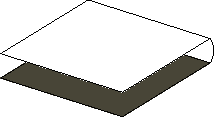
\includegraphics[width=.9\textwidth]{sam_images/checkerboard-3d.pdf}

\end{columns}

\end{frame}

%%%%%%%%%%%%%%%%%%%%%%%%%%%%%%%%%%%%%%%%%%%%%%%%%%%%%%%%%%%%%%%%%%%%%%%%

\begin{frame}
\frametitle{Partial Ordering}
\begin{block}{Goal:}
Use checkerboard pattern and crease assignments to tell, for each pair of adjacent faces, which face comes first in \textit{all} linear orderings.
\end{block}

\bigskip

\begin{columns}[c]
\column{.45\textwidth}
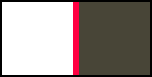
\includegraphics[width=\textwidth]{sam_images/cboard-valley-tile.pdf}

\pause

\column{.45\textwidth}
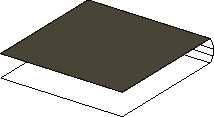
\includegraphics[width=.9\textwidth]{sam_images/checkerboard-3a.pdf}

\end{columns}

\end{frame}

%%%%%%%%%%%%%%%%%%%%%%%%%%%%%%%%%%%%%%%%%%%%%%%%%%%%%%%%%%%%%%%%%%%%%%%%

\begin{frame}
\frametitle{Partial Ordering}
\begin{block}{Goal:}
Use checkerboard pattern and crease assignments to tell, for each pair of adjacent faces, which face comes first in \textit{all} linear orderings.
\end{block}

\bigskip

\begin{columns}[c]

\column{.45\textwidth}
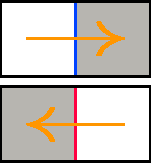
\includegraphics[width=.8\textwidth]{sam_images/checkerboard-tiles.pdf}

\pause

\column{.45\textwidth}
\includegraphics[width=\textwidth]{sam_images/cp-w-cboard.pdf}

\end{columns}

\end{frame}

%%%%%%%%%%%%%%%%%%%%%%%%%%%%%%%%%%%%%%%%%%%%%%%%%%%%%%%%%%%%%%%%%%%%%%%%

\begin{frame}
\frametitle{Partial Ordering}
\begin{block}{Goal:}
Use checkerboard pattern and crease assignments to tell, for each pair of adjacent faces, which face comes first in \textit{all} linear orderings.
\end{block}

\bigskip

\begin{columns}[c]

\column{.45\textwidth}
\includegraphics[width=.8\textwidth]{sam_images/checkerboard-tiles.pdf}

\column{.45\textwidth}
\includegraphics[width=\textwidth]{sam_images/cp-w-cboard-and-dag.pdf}

\end{columns}

\end{frame}
%%%%%%%%%%%%%%%%%%%%%%%%%%%%%%%%%%%%%%%%%%%%%%%%%%%%%%%%%%%%%%%%%%%%%%%%
\begin{frame}

\frametitle{Linear Orderings}
Is satisfying this partial ordering enough to ensure foldability? \pause \textbf{No!}

\pause
\bigskip

\begin{columns}[c]
\column{.45\textwidth}
\includegraphics[width=\textwidth]{sam_images/bad-butterfly.pdf}
\end{columns}

\end{frame}
%%%%%%%%%%%%%%%%%%%%%%%%%%%%%%%%%%%%%%%%%%%%%%%%%%%%%%%%%%%%%%%%%%%%%%%%

\begin{frame}
\frametitle{Butterflies}

\begin{columns}[c]

\column{.45\textwidth}
\includegraphics[width=\textwidth]{sam_images/map-w-butterfly-1.pdf}

\column{.45\textwidth}
\includegraphics[width=\textwidth]{sam_images/checkerboard-3a.pdf}

\end{columns}

\end{frame}

%%%%%%%%%%%%%%%%%%%%%%%%%%%%%%%%%%%%%%%%%%%%%%%%%%%%%%%%%%%%%%%%%%%%%%%%

\begin{frame}
\frametitle{Butterflies}

\begin{columns}[c]

\column{.45\textwidth}
\includegraphics[width=\textwidth]{sam_images/map-w-butterfly-2.pdf}

\pause

\column{.45\textwidth}
\includegraphics[width=\textwidth]{sam_images/butterfly-big-stack.pdf}

\end{columns}

\end{frame}

%%%%%%%%%%%%%%%%%%%%%%%%%%%%%%%%%%%%%%%%%%%%%%%%%%%%%%%%%%%%%%%%%%%%%%%%

\begin{frame}
\frametitle{Butterfly Condition}

\begin{block}{Goal:}
Enumerate the realizable configurations of \textit{twin butterfly} pairs.
\end{block}

\bigskip

\begin{columns}[c]
\column{.45\textwidth}
\includegraphics[width=\textwidth]{sam_images/butterfly-big-stack.pdf}

\end{columns}

\end{frame}

%%%%%%%%%%%%%%%%%%%%%%%%%%%%%%%%%%%%%%%%%%%%%%%%%%%%%%%%%%%%%%%%%%%%%%%%

\begin{frame}
\frametitle{Butterfly Condition}

\begin{block}{Goal:}
Enumerate the realizable configurations of twin butterfly pairs.
\end{block}

\bigskip

\begin{columns}[c]
\column{.45\textwidth}
\includegraphics[width=\textwidth]{sam_images/butterfly-stack.pdf}

\pause

\column{.45\textwidth}
\includegraphics[width=\textwidth]{sam_images/butterfly-nest.pdf}

\end{columns}

\end{frame}

%%%%%%%%%%%%%%%%%%%%%%%%%%%%%%%%%%%%%%%%%%%%%%%%%%%%%%%%%%%%%%%%%%%%%%%%

\begin{frame}
\frametitle{Butterfly Condition}

\begin{block}{Goal:}
Enumerate the realizable configurations of twin butterfly pairs.
\end{block}

\bigskip

\begin{columns}[c]
\column{.45\textwidth}
\includegraphics[width=\textwidth]{sam_images/bad-butterfly.pdf}

\end{columns}

\end{frame}

%%%%%%%%%%%%%%%%%%%%%%%%%%%%%%%%%%%%%%%%%%%%%%%%%%%%%%%%%%%%%%%%%%%%%%%%

\subsection{Formal Proof}

\begin{frame}
\frametitle{Conditions for flat-foldability}

\begin{block}{Theorem:}
A linear ordering $\O$ of faces is flat-foldable if and only if $(i)$ $\O$ satisfies the partial ordering given by the map and $(ii)$ every pair of twin butterflies stacks or nests in $\O$. 
\end{block}

\medskip

\pause

\textit{Proof}: $[\implies]$ We have already proven this direction.

\medskip

\begin{columns}[c]

\pause

\column{.3\textwidth}
\includegraphics[width=\textwidth]{sam_images/checkerboard-tiles.pdf}

\pause

\column{.3\textwidth}
\includegraphics[width=.8\textwidth]{sam_images/butterfly-stack.pdf}

\bigskip
\includegraphics[width=.8\textwidth]{sam_images/butterfly-nest.pdf}

\column{.4\textwidth}
\includegraphics[width=.7\textwidth]{sam_images/bad-butterfly.pdf}

\end{columns}

\end{frame}

%%%%%%%%%%%%%%%%%%%%%%%%%%%%%%%%%%%%%%%%%%%%%%%%%%%%%%%%%%%%%%%%%%%%%%%%

\begin{frame}
\frametitle{Conditions for flat-foldability}

\begin{block}{Theorem: (Nishat and Whitesides)}
A linear ordering $\O$ of faces is flat-foldable if and only if $(i)$ $\O$ satisfies the partial ordering given by the map and $(ii)$ every pair of twin butterflies stacks or nests in $\O$. 
\end{block}

\medskip

\textit{Proof}: $[\impliedby]$ Let's prove this direction now.

\medskip

\begin{columns}[c]

\pause

\column{.3\textwidth}
\includegraphics[width=\textwidth]{sam_images/linear-order-faces.pdf}

\pause

\column{.3\textwidth}
\includegraphics[width=\textwidth]{sam_images/2x2-map-folded.pdf}

\end{columns}

\end{frame}

%%%%%%%%%%%%%%%%%%%%%%%%%%%%%%%%%%%%%%%%%%%%%%%%%%%%%%%%%%%%%%%%%%%%%%%%

\begin{frame}
\frametitle{Computational Complexity of Validity Testing}

Algorithm for determining whether or not a linear ordering is valid:

\pause

\begin{enumerate}
\item Check that the linear ordering satisfies the partial ordering given by the map.
\pause
\item Check that every pair of twin butterflies stacks or nests.
\end{enumerate}

\bigskip

\pause
This can be done in $\mathcal{O}(mn)$ (linear) time, which is super fast!

\bigskip

\pause

\textbf{Summary:} If someone says ``This map can be flat-folded, here is the folding,'' we can quickly test whether or not they were correct.

\end{frame}

%%%%%%%%%%%%%%%%%%%%%%%%%%%%%%%%%%%%%%%%%%%%%%%%%%%%%%%%%%%%%%%%%%%%%%%%
%%%%%%%%%%%%%%%%%%%%%%%%%%%%%%%%%%%%%%%%%%%%%%%%%%%%%%%%%%%%%%%%%%%%%%%%
%%%%%%%%%%%%%%%%%%%%%%%%%%%%%%%%%%%%%%%%%%%%%%%%%%%%%%%%%%%%%%%%%%%%%%%%
%%%%%%%%%%%%%%%%%%%%%%%%%%%%%%%%%%%%%%%%%%%%%%%%%%%%%%%%%%%%%%%%%%%%%%%%
%%%%%%%%%%%%%%%%%%%%%%%%%%%%%%%%%%%%%%%%%%%%%%%%%%%%%%%%%%%%%%%%%%%%%%%%
%%%%%%%%%%%%%%%%%%%%%%%%%%%%%%%%%%%%%%%%%%%%%%%%%%%%%%%%%%%%%%%%%%%%%%%%

\section{Meanders}

\newcommand{\R}{\mathsf{R}}
\renewcommand{\L}{\mathsf{L}}


\begin{frame}
\frametitle{Counting Problems in Origami}
\begin{itemize}
\item How many ways can we fold an $n\times m$ map?
	\begin{itemize}
	\item How many ways can we fold a $1\times m$ map?
	\end{itemize}
\item How many $n\times m$ map crease patterns can be folded, period?
	\begin{itemize}
	\item How many ways can we fold a $1\times m$ map?
	\end{itemize}
\end{itemize}
\end{frame}

\begin{frame}
\frametitle{Star Patterns}
\begin{center}
\includegraphics[width=.8\textwidth]{meanders/star-cp.pdf}
\end{center}
\pause
\textbf{Question:} How many foldings are generated by star patterns with $2n$ creases?
\end{frame}

\begin{frame}
\frametitle{Representing foldings of Star Patterns}
\begin{center}
\includegraphics[width=\textwidth]{meanders/star-to-meander.pdf}
\end{center}

\end{frame}

\begin{frame}
\frametitle{Examples of Meanders}
\begin{center}
\includegraphics[width=.8\textwidth]{meanders/12-and-3.pdf}
\end{center}

\end{frame}

\begin{frame}
\frametitle{Examples of Meanders}
\begin{center}
\includegraphics[width=.8\textwidth]{meanders/order-10.pdf}
\end{center}

\end{frame}

\begin{frame}
\frametitle{Examples of Meanders}
\begin{table}
\begin{tabular}{c c}
\toprule
\textbf{Order $n$} & \textbf{\# Meanders $M_n$}\\
\midrule
1 & 1 \\
2 & 2 \\
3 & 8 \\
4 & 42 \\
5 & 262 \\
\vdots & \vdots\\
\pause
10 & \pause 8,152,860 \\
\vdots & \vdots\\
\bottomrule
\end{tabular}
\caption{The sequence of Meandric Numbers}
\end{table}
\end{frame}

\begin{frame}
\frametitle{Game Plan}
\begin{center}
\includegraphics[width=.8\textwidth]{meanders/1-with-2.pdf}
\end{center}
\end{frame}

\subsection{Our Method}

\begin{frame}
\frametitle{Game Plan}
\begin{center}
\includegraphics[width=.8\textwidth]{meanders/1-into-2.pdf}
\end{center}
\pause
\textbf{Idea:} Produce larger meanders by adding ``twists'' to smaller meanders
\end{frame}

\begin{frame}
\frametitle{Will it work?}
\begin{center}
\includegraphics[width=\textwidth]{meanders/2-into-3_1.pdf}
\end{center}
\end{frame}

\begin{frame}
\frametitle{Will it work?}
\begin{center}
\includegraphics[width=\textwidth]{meanders/2-into-3_2.pdf}
\end{center}
\end{frame}

\begin{frame}
\frametitle{Will it work?}
\begin{center}
\includegraphics[width=\textwidth]{meanders/2-into-3_3.pdf}
\end{center}
\end{frame}

\begin{frame}
\frametitle{Will it work?}
\begin{center}
\includegraphics[width=\textwidth]{meanders/2-into-3_4.pdf}
\end{center}
\end{frame}

\begin{frame}
\frametitle{Will it work?}
\textbf{Question:} Can we get all meanders by repeatedly doing this?
\pause
\textbf{Answer:} Sadly we cannot:

\begin{center}
\includegraphics[width=.4\textwidth]{meanders/5-example.pdf}
\end{center}

\end{frame}

\begin{frame}
\frametitle{Will it work?}
\begin{center}
\includegraphics[width=\textwidth]{meanders/5-shuffle.pdf}
\end{center}

\end{frame}

\begin{frame}
\frametitle{Meanders}
\begin{theorem}
All meanders may be built from $m_1 = \circ$ with at most one shuffle after each twist.
\end{theorem}
\end{frame}

\begin{frame}
\frametitle{Simple Meanders}
\begin{definition}[Simple Meander]
A \emph{simple meander} is a meander of order $n$ that can be constructed without shuffling.
\end{definition}
\end{frame}

\begin{frame}
\frametitle{Simple Meanders}
\renewcommand{\P}{\mathbb{P}}

\begin{theorem}[Recurrence Relation for Simple Meanders]
Let $\P(k,n) = \{(x_1,x_2,\ldots,x_n) : \sum x_i = k \text{ and } x_i\ge 0 \forall i\}$. Then
\begin{align*}
r(n) &= \sum_{i=1}^n\sum_{P\in\P(i,n+1)}\prod^{n+1}_{k = 1} r(P_k)\\
H(n) &= \sum_{i=1}^n r(i) \sum_{P\in\P(i,n)}\prod^{n}_{k = 1} H(P_k)\\
M^s_n &= 2H(n)
\end{align*}
\end{theorem}
\end{frame}

%____________________________________%
%_______ EXAMPLE SLIDES BELOW _______%
%________________ || ________________%
%_________________V__________________%

% \begin{frame}[fragile] % Need to use the fragile option when verbatim is used in the slide
% \frametitle{Citation}
% An example of the \verb|\cite| command to cite within the presentation:\\~

% This statement requires citation \cite{p1}.
% \end{frame}

%------------------------------------------------

\begin{frame}
\frametitle{References}
\footnotesize{
\begin{thebibliography}{99} % Beamer does not support BibTeX so references must be inserted manually as below
\bibitem[Smith, 2012]{p1} John Smith (2012)
\newblock Title of the publication
\newblock \emph{Journal Name} 12(3), 45 -- 678.
\end{thebibliography}
}
\end{frame}

%------------------------------------------------

\begin{frame}
\Huge{\centerline{Q.E.D.}}
\end{frame}

%---------------------------------------------------

\end{document}